\documentclass{standalone}
\usepackage{graphicx}	
\usepackage{amssymb, amsmath, amsthm}
\usepackage{color}

\usepackage{tikz}
\usetikzlibrary{math, arrows.meta}

\definecolor{light}{RGB}{220, 188, 188}
\definecolor{mid}{RGB}{185, 124, 124}
\definecolor{dark}{RGB}{143, 39, 39}
\definecolor{highlight}{RGB}{180, 31, 180}
\definecolor{darkteal}{RGB}{29, 79, 79}
\definecolor{darkolive}{RGB}{97, 123, 45}
\definecolor{gray10}{gray}{0.1}
\definecolor{gray20}{gray}{0.2}
\definecolor{gray30}{gray}{0.3}
\definecolor{gray40}{gray}{0.4}
\definecolor{gray60}{gray}{0.6}
\definecolor{gray70}{gray}{0.7}
\definecolor{gray80}{gray}{0.8}
\definecolor{gray90}{gray}{0.9}
\definecolor{gray95}{gray}{0.95}

\begin{document}

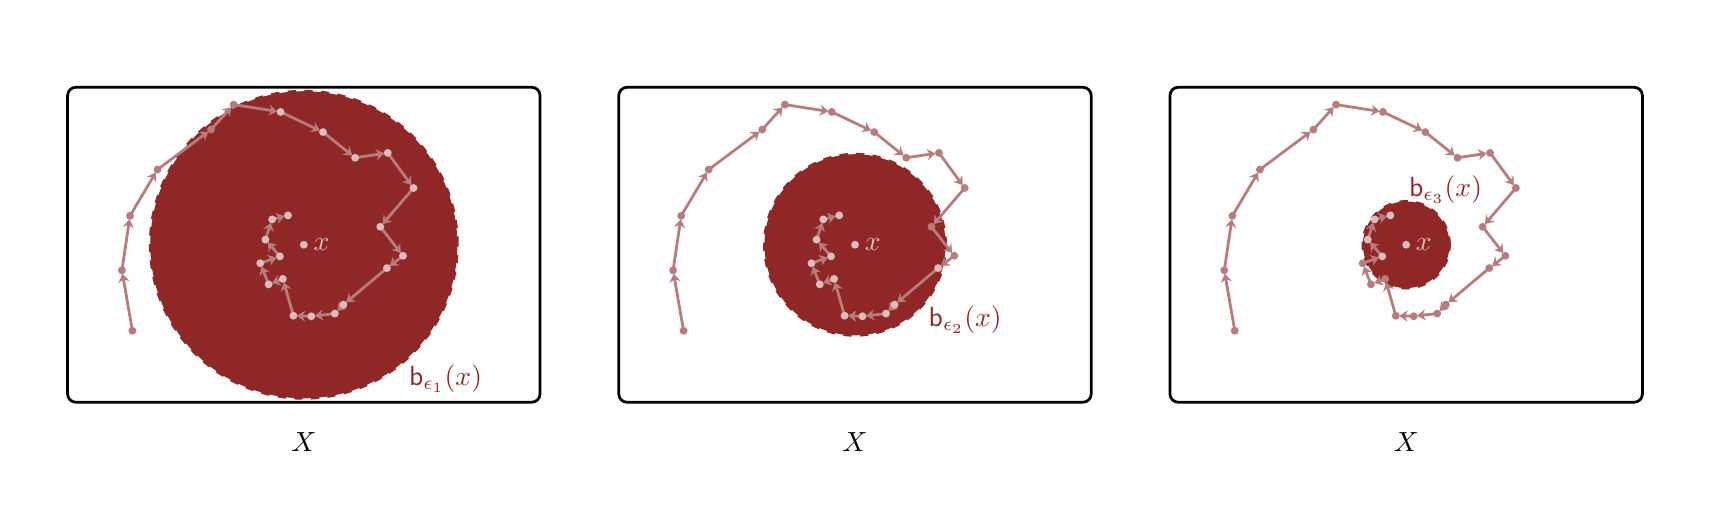
\begin{tikzpicture}[scale=1.0]
  
  \pgfmathsetmacro{\m}{7}
  \pgfmathsetmacro{\eps}{1.95}
   
  \begin{scope}[shift={(0, 0)}]
    \draw[white] (-3.5, -3) rectangle (3.5, 2.75);
  
    \draw[rounded corners=3, color=black, line width=1] (-3, -2) rectangle (3, 2);
    \node at (0, -2.5) { $X$ };

    \filldraw[dark, dashed, line width=1] (0, 0) circle(\eps);
    \node[dark] at (1.8, -1.7) { $\mathsf{b}_{\epsilon_{1}}(x)$ };
  
    \foreach [count=\n] \x/\y in {-2.177/-1.092, -2.310/-0.325, -2.207/0.368, -1.858/0.955, -1.178/1.463, 
                                  -0.891/1.780, -0.295/1.687, 0.244/1.431, 0.651/1.105, 1.066/1.167, 
                                  1.393/0.721, 0.971/0.228, 1.260/-0.140, 1.056/-0.296, 0.503/-0.760, 
                                  0.394/-0.874, 0.095/-0.908, -0.132/-0.901, -0.266/-0.434, -0.447/-0.503, 
                                  -0.553/-0.235, -0.304/-0.147, -0.488/0.065, -0.402/0.322, -0.201/0.373} {
      \ifnum \n>\m
        \colorlet{pointcolor}{light}; 
      \else
        \colorlet{pointcolor}{mid};
      \fi
      
      \ifnum \n>1
        \draw[color=mid, -{Stealth[length=3, width=4]}, 
              line width=1, shorten >=1.25] (A) -- (\x, \y);
        \fill[color=pointcolor] (A) circle (0.05);
      \fi
    
      \ifnum \n=25
        \fill[color=pointcolor] (\x, \y) circle (0.05);
      \fi
      \coordinate (A) at (\x, \y);
    }
    
    \fill[light] (0, 0) circle (0.05) node[right] { $x$ };
  \end{scope}
    
  \pgfmathsetmacro{\m}{14}
  \pgfmathsetmacro{\eps}{1.15}
  
  \begin{scope}[shift={(7, 0)}]
    \draw[white] (-3.5, -3) rectangle (3.5, 2.75);
  
    \draw[rounded corners=3, color=black, line width=1] (-3, -2) rectangle (3, 2);
    \node at (0, -2.5) { $X$ };
      
    \filldraw[dark, dashed, line width=1] (0, 0) circle(\eps);
    \node[dark] at (1.4, -0.95) { $\mathsf{b}_{\epsilon_{2}}(x)$ };
  
    \foreach [count=\n] \x/\y in {-2.177/-1.092, -2.310/-0.325, -2.207/0.368, -1.858/0.955, -1.178/1.463, 
                                  -0.891/1.780, -0.295/1.687, 0.244/1.431, 0.651/1.105, 1.066/1.167, 
                                  1.393/0.721, 0.971/0.228, 1.260/-0.140, 1.056/-0.296, 0.503/-0.760, 
                                  0.394/-0.874, 0.095/-0.908, -0.132/-0.901, -0.266/-0.434, -0.447/-0.503, 
                                  -0.553/-0.235, -0.304/-0.147, -0.488/0.065, -0.402/0.322, -0.201/0.373} {
      \ifnum \n>\m
        \colorlet{pointcolor}{light}; 
      \else
        \colorlet{pointcolor}{mid};
      \fi
      
      \ifnum \n>1
        \draw[color=mid, -{Stealth[length=3, width=4]}, 
              line width=1, shorten >=1.25] (A) -- (\x, \y);
        \fill[color=pointcolor] (A) circle (0.05);
      \fi
    
      \ifnum \n=25
        \fill[color=pointcolor] (\x, \y) circle (0.05);
      \fi
      \coordinate (A) at (\x, \y);
    }
    
    \fill[light] (0, 0) circle (0.05) node[right] { $x$ };
  \end{scope}

  \pgfmathsetmacro{\m}{22}
  \pgfmathsetmacro{\eps}{0.55}
    
  \begin{scope}[shift={(14, 0)}]
    \draw[white] (-3.5, -3) rectangle (3.5, 2.75);
  
    \draw[rounded corners=3, color=black, line width=1] (-3, -2) rectangle (3, 2);
    \node at (0, -2.5) { $X$ };
      
    \filldraw[dark, dashed, line width=1] (0, 0) circle(\eps);
    \node[dark] at (0.5, 0.7) { $\mathsf{b}_{\epsilon_{3}}(x)$ };
  
    \foreach [count=\n] \x/\y in {-2.177/-1.092, -2.310/-0.325, -2.207/0.368, -1.858/0.955, -1.178/1.463, 
                                  -0.891/1.780, -0.295/1.687, 0.244/1.431, 0.651/1.105, 1.066/1.167, 
                                  1.393/0.721, 0.971/0.228, 1.260/-0.140, 1.056/-0.296, 0.503/-0.760, 
                                  0.394/-0.874, 0.095/-0.908, -0.132/-0.901, -0.266/-0.434, -0.447/-0.503, 
                                  -0.553/-0.235, -0.304/-0.147, -0.488/0.065, -0.402/0.322, -0.201/0.373} {
      \ifnum \n>\m
        \colorlet{pointcolor}{light}; 
      \else
        \colorlet{pointcolor}{mid};
      \fi
      
      \ifnum \n>1
        \draw[color=mid, -{Stealth[length=3, width=4]}, 
              line width=1, shorten >=1.25] (A) -- (\x, \y);
        \fill[color=pointcolor] (A) circle (0.05);
      \fi
    
      \ifnum \n=25
        \fill[color=pointcolor] (\x, \y) circle (0.05);
      \fi
      \coordinate (A) at (\x, \y);
    }
    
    \fill[light] (0, 0) circle (0.05) node[right] { $x$ };
  \end{scope}
    
\end{tikzpicture}

\end{document}  